%%%%%%%%%%%%%%%%%%%%%%%%%%%%%%%%%%%%%%%%%%%%%%%%%%%%%%%%%%
%%% Section 5: Exploration
%%%%%%%%%%%%%%%%%%%%%%%%%%%%%%%%%%%%%%%%%%%%%%%%%%%%%%%%%%

\section{Exploration of Energy Storage Sizing} \label{section:exploration}

% This section first shows an exploration of how to improve forward progress by sizing energy storage with respect to supply current and volatile state size (Section~\ref{subsec:sizees}), and then demonstrates the sizing approach for energy storage in real-world energy source conditions. The sizing method finds the suitable energy harvester size that achieves a target forward progress and explores the energy storage sizing effect (Section~\ref{subsec:harvstor}), with a trade-off in forward progress, capacitor volume, and interruption periods (Section~\ref{subsec:tradeoff}).

In this section, we configure the reactive ICS model presented in Section~\ref{section:model} to approximate a real ICS platform, and then present an exploration of the relationship between $\alpha_{exe}$ and $C$ with respect to $I_{harv}$ and volatile state size.

\subsection{Model Configuration}

\subsubsection{Energy Storage}

The energy storage is represented as an ideal capacitor with leakage current. Its terminal voltage is directly applied to the load, so is modelled as:
\begin{equation}
  C \frac{dV_{cc}}{dt} = I_{harv} - I_{load} - I_{leak}
\end{equation}
where $I_{load}$ is the current consumption of the load. In this exploration, we refer to the empirical $I_{leak}$ of AVX TAJ low-profile series tantalum capacitors, which depends on capacitance $C$, rated voltage $V_{rated}$, and terminal voltage $V_{cc}$~\cite{avxleakage}:
% an off-the-shelf tantalum capacitor~\cite{tancap1}
\begin{equation}
    % aluminium 
%   I_{leak} = max\{0.03 C V_{rated}, \quad 4 \times 10^{-6}\}    \quad (A)
    % tantalum
    I_{leak} = 0.01 \lambda C V_{rated} \quad (A)
\end{equation}
where $\lambda$ denotes the ratio of the actual current leakage at $V_{cc}$ to the current leakage at $V_{rated}$, and $\lambda$ is approximated as: 
\begin{equation}
    \lambda = 0.05 \times 20^{\frac{V_{cc}}{V_{rated}}}
\end{equation}
We assume a typical load of $<$ \SI{4.0}{\volt} so, to minimize leakage, we select a device with $V_{rated} =$ \SI{10}{\volt} so as to operate between 25-40\% of its rated voltage~\cite{avxleakage}. 

% Here, $V_{cc}$ affects both the energy harvester and the load. On the harvester side, $V_{cc}$ is the operating voltage of PV cells, which has an effect on the harvested current $I_{harvest}$. On the load side, $V_{cc}$ is the supply voltage, which determines when the load wakes up or powers off (affecting $I_{load}$). Hence, the energy storage, the energy harvester, and the load impact on each other through $V_{cc}$, $I_{harvest}$, and $I_{load}$. 

\subsubsection{Intermittent Computing Load} \label{ssubsec:loadconfig}

The load parameters of current draws and time overheads, as listed in Table~\ref{tab:load}, were profiled with the experimental settings explained in Section~\ref{section:experiment}. 
The current draw was profiled with experimental measurements at a range of supply voltages. The variation of $I_{lpm}$ between $V_{off}$ (\SI{1.8}{\volt}) and $V_{r}$ (\SI{2.4}{\volt}) is 2\%, and for $I_{exe}$ between $V_{s}$ (\SI{2.1}{\volt}) and \SI{3.3}{\volt} is 1.5\%. $I_{exe}$ also has a run-time variation of 2.8\% due to a variable memory access rate. We omit these minor variations and use the mean of $I_{exe}$ and $I_{lpm}$ in the model. $I_{r}$ and $I_{s}$ are measured at $V_{r}$ and $V_{s}$ respectively. Given the voltage thresholds and the current consumption, the minimum energy storage capacitance is \SI{6.2}{\micro\farad}. This guarantees that a save and restore operation can complete even if the incoming supply current drops instantaneously to zero. The model parameters in Table~\ref{tab:load} are given as an example, and can be changed for different load characteristics. For example, $T_{r}$ and $T_{s}$ can be tuned for different volatile state sizes.
% $I_{exe}$ also has a run-time variation of \SIrange{-2.4}{+2.8}{\percent} 

\begin{table}[!t]
    \renewcommand{\arraystretch}{1.2}
    \centering
    \caption{Profiled MCU parameters}
    \label{tab:load}
    \begin{tabular}{|c|c|}
    \hline
    \textbf{Parameter} & \textbf{Value}\\
    \hline
    $I_{exe}$ & \SI{887}{\micro\ampere}\\
    $I_{lpm}$ & \SI{26}{\micro\ampere}\\
    $I_{r}$ & \SI{971}{\micro\ampere}\\
    $I_{s}$ & \SI{811}{\micro\ampere}\\
    $T_{r}$ & \SI{1.903}{\milli\second}\\
    $T_{s}$ & \SI{1.880}{\milli\second}\\
    % \multicolumn{2}{c}{Measured Parameters}\\
    % \hline
    % $I_{exe}, I_{R}, I_{S}$ & 0.87 mA\\
    % $I_{lpm}$ & 0.40 mA\\
    % $T_{r}$ & 2.298 ms\\
    % $T_{s}$ & 2.274 ms\\
    % \hline
    % \multicolumn{2}{c}{Simulation Parameters}\\
    % \hline
    % $I_{exe}, I_{R}, I_{S}$ & 1.00 mA\\
    % $I_{lpm}$ & 0.01 mA\\
    \hline
    \end{tabular}
\end{table}



\subsection{Sizing Energy Storage to Improve Forward Progress} \label{subsec:sizees}

% Message/Summary, How, Results. 

\subsubsection{Impact of Supply Current}

Increasing energy storage capacitance above the minimum can improve forward progress by reducing the frequency of power interruptions, but this improvement may be offset by increased leakage. \figurename{~\ref{fig:fpwconstcurr}} shows the relationship between forward progress and energy storage capacitance for a range of constant supply currents. Optimal capacitance values are shown for each current value.
% Forward progress increases with energy storage capacitance. However, , which leads to an optimal storage capacitance. 

% some more explanation about details in this graph
The minimum capacitance (dashed line in \figurename{~\ref{fig:fpwconstcurr}}) is calculated to deliver correct operation even if the supply current instantaneously drops to zero. If it does not drop to zero, this means that correct operation could have continued even with a smaller capacitance, though designing a system in this way would be inadvisable owing to unpredictability of the supply. This property is illustrated in \figurename{~\ref{fig:fpwconstcurr}}, in the area on the left of the dashed line. It may be observed that, for each of the current values, there is a sudden drop-off towards zero forward progress. This illustrates the hazard of setting the capacitance too small: the stored energy is too low to allow a restore and save to be undertaken.
%This steep fall is because the implemented control algorithm enters the low-power mode with volatile state retained after a save operation, and hence the energy used for restoring state in the first operating cycle is then used for effective execution in the following operating cycles as long as the supply voltage recovers to the restore threshold without a power interruption.
 
 % ), the execution may still progress given that the current supply keeps providing energy during execution
Typically, commercially-available capacitors have a $\pm$20\% tolerance. The effect of this variation on maximum forward progress is shown to be negligible ($<$ 0.23\%) in \figurename{~\ref{fig:fpwconstcurr}}. However, it must be pointed out that the effect would be much more pronounced if operating at the minimum capacitance as the variation of forward progress is larger with smaller capacitance values. Thus, it is recommended that a tolerance is considered when designing ICSs with minimum capacitance.

%If the volatile state is not retained in low-power mode (i.e. necessary to restore every operating cycle) or the supply only lasts for a limited period, 

% red zone: when supply current doesn't last for long. 
% (Regarding the red zone, potentially show a graph of the number of operating cycles to approximate constant current supply.)

\begin{figure}[!t]
  \centering
  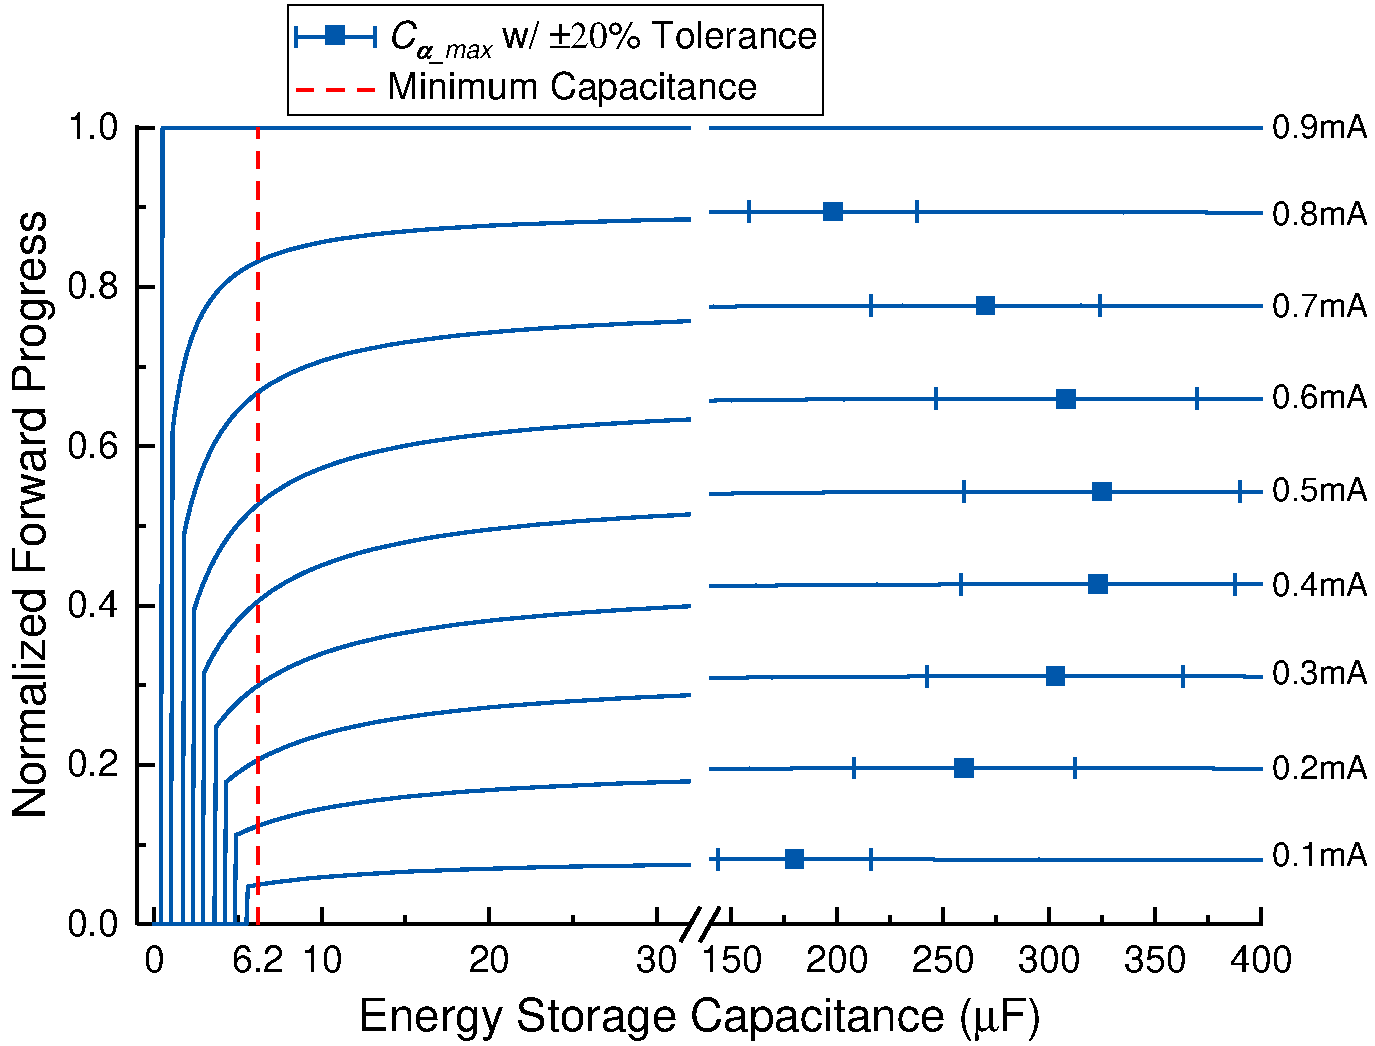
\includegraphics[width=3.2in]{ch3_sizingeffect/figures/StorCCur6Fig} 
  \caption{Forward progress against energy storage capacitance at different levels of constant supply current. Error bars around optimal points denote the impact of typical $\pm$20\% capacitance tolerance. }
  \label{fig:fpwconstcurr}
\end{figure}

\begin{figure}[!t]
  \centering
  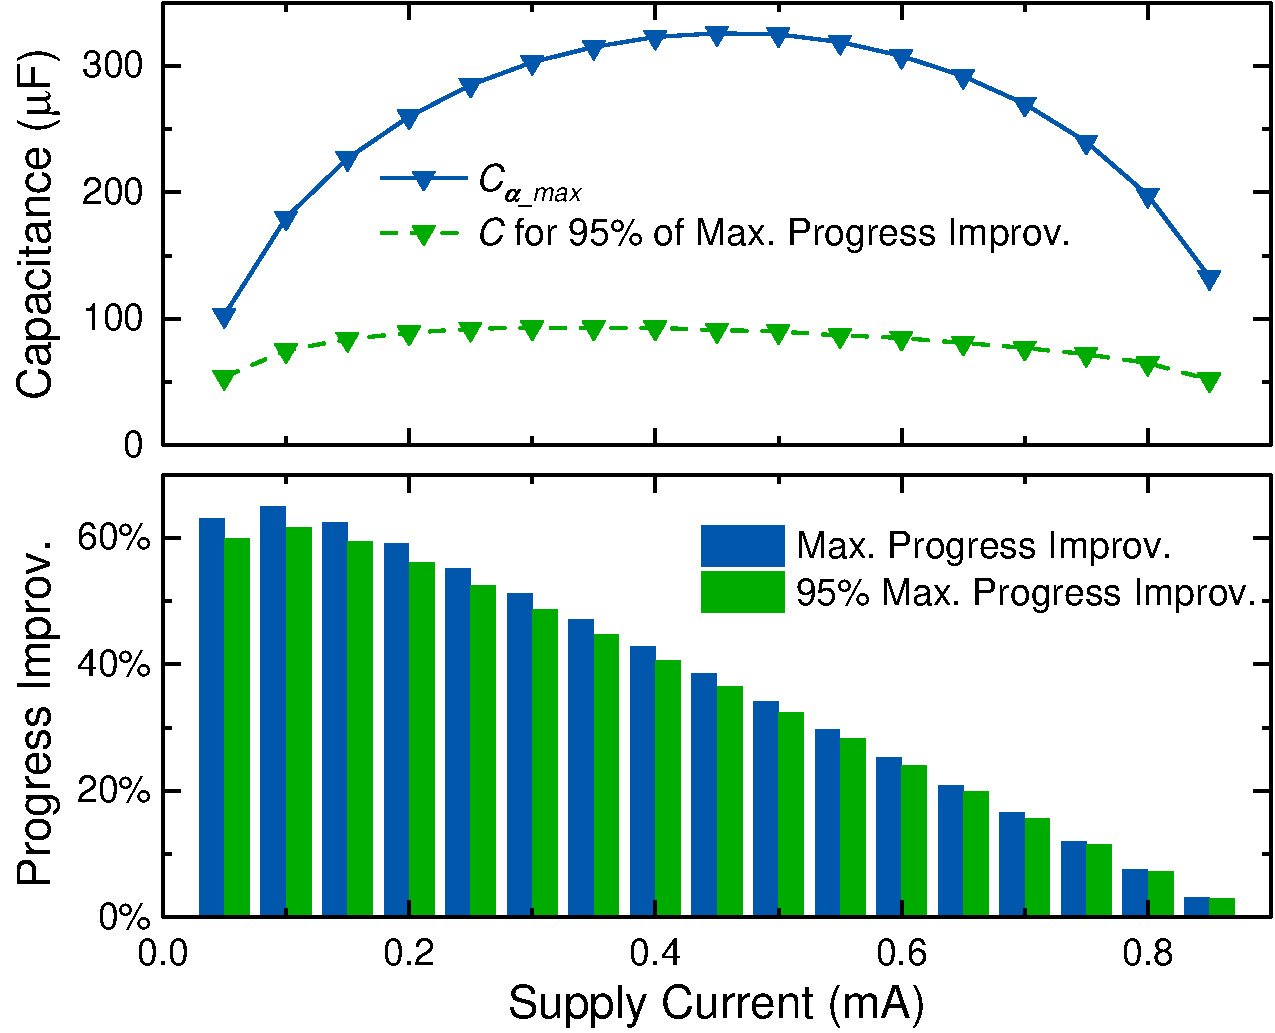
\includegraphics[width=3.2in]{ch3_sizingeffect/figures/StorCCurMax4Fig}
  \caption{Maximum forward progress improvement by sizing energy storage given a spectrum of supply current (normalized by the minimum capacitance case), with the corresponding maximum and sub-maximum (95\% of maximum) capacitance. }
  \label{fig:maxfwp}
\end{figure}

\figurename{~\ref{fig:maxfwp}} shows that an improvement in forward progress of up to 65\%  can be achieved when using the optimal capacitance instead of the minimum. However, it may not be desirable to set the capacitance solely for maximizing forward progress, because there are often trade-offs with other factors including increased interruption periods and dimensions. 
% (explored in Section~\ref{subsec:tradeoff}).
% In real-world energy source conditions, the supply current varies across this spectrum, and hence leads to an overall progress improvement based on its supply distribution. 
% This improvement exists only when the device operates in the Intermittent mode, since the device keeps either inactive in the Off mode or active in the On mode without the need for restoring and saving state. 
% Correspondingly, the optimal energy storage capacity is also plotted against supply current. 
% This optimal capacity exists because of the side effect of capacitor leakage; without capacitor leakage effect, the forward progress would keep approaching the ideal case (as explained in Section~\ref{subsec:formulation}). 
While a large improvement can be delivered with the optimal capacitance, as shown in \figurename{~\ref{fig:maxfwp}}, 95\% of this gain can still be obtained with significantly smaller capacitances (mean 31\% of the optimal value).
For example, reducing from \SI{325}{\micro\farad} to \SI{90}{\micro\farad} gives 95\% of the maximum improvement with a \SI{0.5}{\milli\ampere} supply. 

% in real deployment, storage fixed while current varies, change over a range, we may need to pick a capacity that optimise the majority of energy conditions. 

\subsubsection{Impact of Volatile State Size}

The size of volatile state differs across applications with different amounts of RAM usage, and hence incurs varying time and energy overheads for restore and save operations. We measured time overheads of restore and save operations in the minimum case (64B register data and a 160B stack) and the maximum case (64B register data and a full 2048B RAM) respectively as shown in Table~\ref{tab:ramscale}. As these time overheads are expected to be linear to the state size~\cite{Sliper:2019:ESR:3316781.3317812}, the model can be tuned for various volatile state sizes by linearly scaling the profiled values. 

% In the MCU we explore, volatile state includes CPU registers and SRAM data, which takes 64B and 160-2048B. 

\begin{table}[!t]
    \renewcommand{\arraystretch}{1.2}
    \centering
    \caption{Linear scaling range of volatile state size and restore/save time overheads}
    \label{tab:ramscale}
    \begin{tabular}{|c|cc|}
    \hline
    \textbf{State Size} & \multirow{2}{*}{\textbf{Restore Time}} & \multirow{2}{*}{\textbf{Save Time}}\\
    \textbf{(Registers + SRAM)} & & \\
    \hline
    64B + 160B (lower bound) & \SI{232}{\micro\second} & \SI{208}{\micro\second}\\
    % 64B registers + 160B stack
    64B + 2048B (upper bound) & \SI{2.298}{\milli\second} & \SI{2.274}{\milli\second} \\
    % 64B registers + 2048B RAM
    \hline
    \end{tabular}
\end{table}

An example of this is plotted in \figurename{~\ref{fig:ram}}. The forward progress improvement by sizing energy storage increases with the volatile state size, and the optimal capacitance grows accordingly. The improvement becomes insignificant when the volatile state size is small because the restore and save overheads are already negligible. For example, when the workload uses the least volatile state (the leftmost point), the maximum progress improvement is only 3.6\% although the restore and save overheads are reduced by 93\%. 
% This indicates the more efficiently ICSs save/restore, the more useless this work is. 

\begin{figure}[!t]
    \centering
    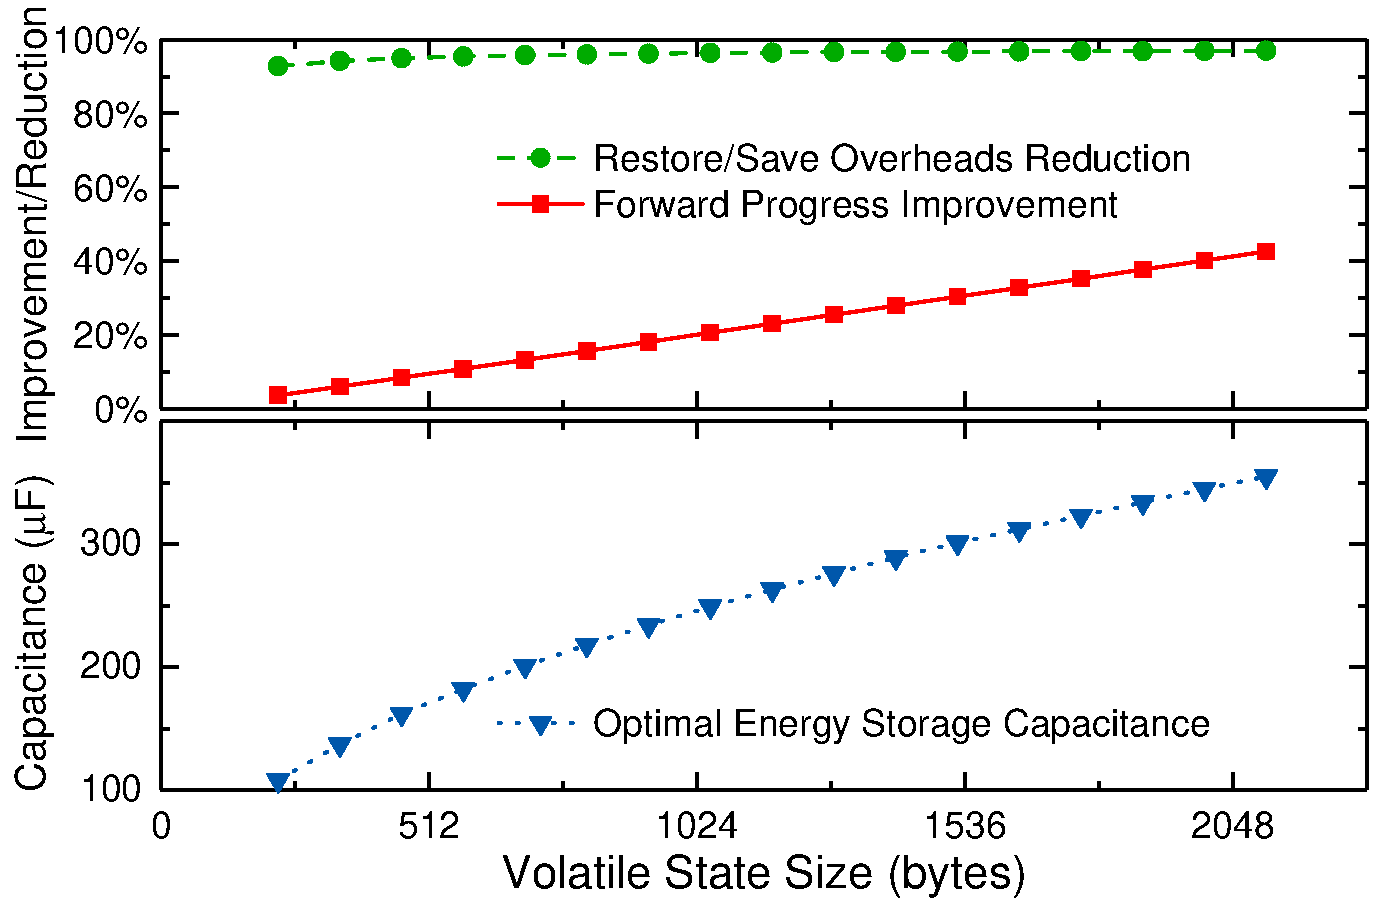
\includegraphics[width=3.2in]{ch3_sizingeffect/figures/RSTORAM3Fig}
    \caption{Impact of RAM usage (linear to restore/save overheads) on sizing energy storage with \SI{0.4}{\milli\ampere} current supply. Improvement and reduction are normalized by the minimum capacitance case. }
    \label{fig:ram}
\end{figure}
